% Created by tikzDevice version 0.12.4 on 2023-06-03 15:48:23
% !TEX encoding = UTF-8 Unicode
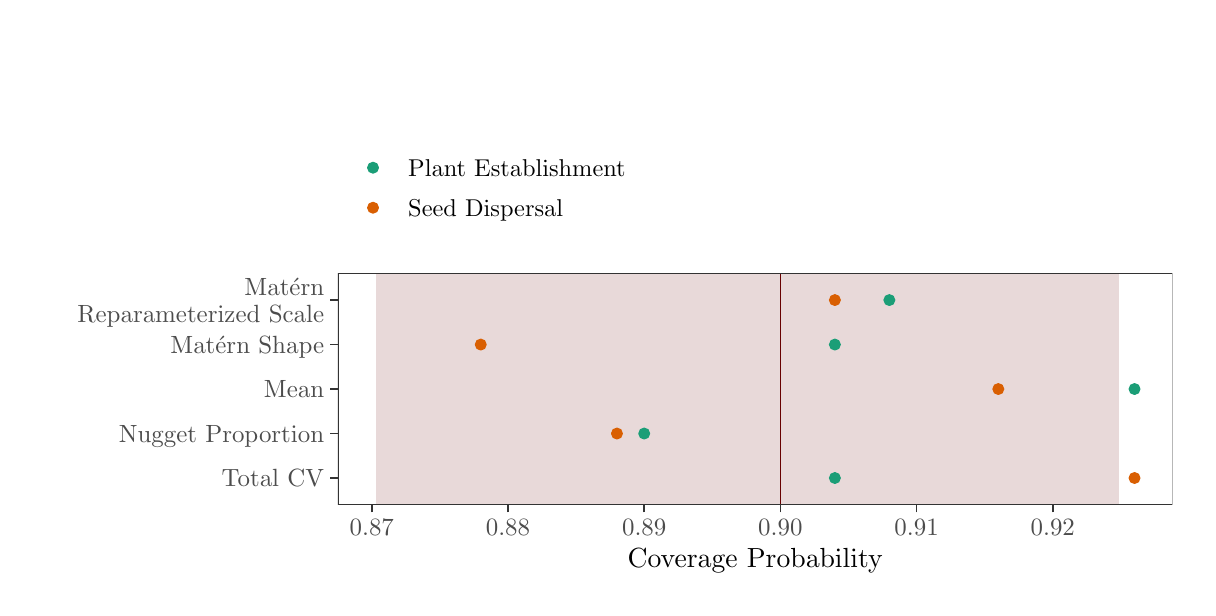
\begin{tikzpicture}[x=1pt,y=1pt]
\definecolor{fillColor}{RGB}{255,255,255}
\path[use as bounding box,fill=fillColor,fill opacity=0.00] (0,0) rectangle (419.17,202.36);
\begin{scope}
\path[clip] (  0.00,  0.00) rectangle (419.17,202.36);
\definecolor{drawColor}{RGB}{255,255,255}
\definecolor{fillColor}{RGB}{255,255,255}

\path[draw=drawColor,line width= 0.6pt,line join=round,line cap=round,fill=fillColor] (  0.00, -0.00) rectangle (419.17,202.36);
\end{scope}
\begin{scope}
\path[clip] (112.07, 29.98) rectangle (413.67,113.58);
\definecolor{fillColor}{RGB}{255,255,255}

\path[fill=fillColor] (112.07, 29.98) rectangle (413.67,113.58);
\definecolor{fillColor}{RGB}{103,0,0}

\path[fill=fillColor,fill opacity=0.15] (125.78, 29.98) rectangle (394.37,113.58);
\definecolor{drawColor}{RGB}{27,158,119}
\definecolor{fillColor}{RGB}{27,158,119}

\path[draw=drawColor,line width= 0.4pt,line join=round,line cap=round,fill=fillColor] (311.37,103.93) circle (  1.96);

\path[draw=drawColor,line width= 0.4pt,line join=round,line cap=round,fill=fillColor] (291.68, 87.85) circle (  1.96);

\path[draw=drawColor,line width= 0.4pt,line join=round,line cap=round,fill=fillColor] (399.96, 71.78) circle (  1.96);

\path[draw=drawColor,line width= 0.4pt,line join=round,line cap=round,fill=fillColor] (222.78, 55.70) circle (  1.96);

\path[draw=drawColor,line width= 0.4pt,line join=round,line cap=round,fill=fillColor] (291.68, 39.63) circle (  1.96);
\definecolor{drawColor}{RGB}{217,95,2}
\definecolor{fillColor}{RGB}{217,95,2}

\path[draw=drawColor,line width= 0.4pt,line join=round,line cap=round,fill=fillColor] (291.68,103.93) circle (  1.96);

\path[draw=drawColor,line width= 0.4pt,line join=round,line cap=round,fill=fillColor] (163.72, 87.85) circle (  1.96);

\path[draw=drawColor,line width= 0.4pt,line join=round,line cap=round,fill=fillColor] (350.74, 71.78) circle (  1.96);

\path[draw=drawColor,line width= 0.4pt,line join=round,line cap=round,fill=fillColor] (212.93, 55.70) circle (  1.96);

\path[draw=drawColor,line width= 0.4pt,line join=round,line cap=round,fill=fillColor] (399.96, 39.63) circle (  1.96);
\definecolor{drawColor}{RGB}{103,0,0}

\path[draw=drawColor,line width= 0.6pt,line join=round] (271.99, 29.98) -- (271.99,113.58);
\definecolor{drawColor}{gray}{0.20}

\path[draw=drawColor,line width= 0.6pt,line join=round,line cap=round] (112.07, 29.98) rectangle (413.67,113.58);
\end{scope}
\begin{scope}
\path[clip] (  0.00,  0.00) rectangle (419.17,202.36);
\definecolor{drawColor}{gray}{0.30}

\node[text=drawColor,anchor=base east,inner sep=0pt, outer sep=0pt, scale=  0.90] at (107.12, 36.53) {Total CV};

\node[text=drawColor,anchor=base east,inner sep=0pt, outer sep=0pt, scale=  0.90] at (107.12, 52.60) {Nugget Proportion};

\node[text=drawColor,anchor=base east,inner sep=0pt, outer sep=0pt, scale=  0.90] at (107.12, 68.68) {Mean};

\node[text=drawColor,anchor=base east,inner sep=0pt, outer sep=0pt, scale=  0.90] at (107.12, 84.76) {Matérn Shape};

\node[text=drawColor,anchor=base east,inner sep=0pt, outer sep=0pt, scale=  0.90] at (107.12,105.69) {Matérn};

\node[text=drawColor,anchor=base east,inner sep=0pt, outer sep=0pt, scale=  0.90] at (107.12, 95.97) {Reparameterized Scale};
\end{scope}
\begin{scope}
\path[clip] (  0.00,  0.00) rectangle (419.17,202.36);
\definecolor{drawColor}{gray}{0.20}

\path[draw=drawColor,line width= 0.6pt,line join=round] (109.32, 39.63) --
	(112.07, 39.63);

\path[draw=drawColor,line width= 0.6pt,line join=round] (109.32, 55.70) --
	(112.07, 55.70);

\path[draw=drawColor,line width= 0.6pt,line join=round] (109.32, 71.78) --
	(112.07, 71.78);

\path[draw=drawColor,line width= 0.6pt,line join=round] (109.32, 87.85) --
	(112.07, 87.85);

\path[draw=drawColor,line width= 0.6pt,line join=round] (109.32,103.93) --
	(112.07,103.93);
\end{scope}
\begin{scope}
\path[clip] (  0.00,  0.00) rectangle (419.17,202.36);
\definecolor{drawColor}{gray}{0.20}

\path[draw=drawColor,line width= 0.6pt,line join=round] (124.34, 27.23) --
	(124.34, 29.98);

\path[draw=drawColor,line width= 0.6pt,line join=round] (173.56, 27.23) --
	(173.56, 29.98);

\path[draw=drawColor,line width= 0.6pt,line join=round] (222.78, 27.23) --
	(222.78, 29.98);

\path[draw=drawColor,line width= 0.6pt,line join=round] (271.99, 27.23) --
	(271.99, 29.98);

\path[draw=drawColor,line width= 0.6pt,line join=round] (321.21, 27.23) --
	(321.21, 29.98);

\path[draw=drawColor,line width= 0.6pt,line join=round] (370.43, 27.23) --
	(370.43, 29.98);
\end{scope}
\begin{scope}
\path[clip] (  0.00,  0.00) rectangle (419.17,202.36);
\definecolor{drawColor}{gray}{0.30}

\node[text=drawColor,anchor=base,inner sep=0pt, outer sep=0pt, scale=  0.90] at (124.34, 18.83) {0.87};

\node[text=drawColor,anchor=base,inner sep=0pt, outer sep=0pt, scale=  0.90] at (173.56, 18.83) {0.88};

\node[text=drawColor,anchor=base,inner sep=0pt, outer sep=0pt, scale=  0.90] at (222.78, 18.83) {0.89};

\node[text=drawColor,anchor=base,inner sep=0pt, outer sep=0pt, scale=  0.90] at (271.99, 18.83) {0.90};

\node[text=drawColor,anchor=base,inner sep=0pt, outer sep=0pt, scale=  0.90] at (321.21, 18.83) {0.91};

\node[text=drawColor,anchor=base,inner sep=0pt, outer sep=0pt, scale=  0.90] at (370.43, 18.83) {0.92};
\end{scope}
\begin{scope}
\path[clip] (  0.00,  0.00) rectangle (419.17,202.36);
\definecolor{drawColor}{RGB}{0,0,0}

\node[text=drawColor,anchor=base,inner sep=0pt, outer sep=0pt, scale=  1.00] at (262.87,  7.44) {Coverage Probability};
\end{scope}
\begin{scope}
\path[clip] (  0.00,  0.00) rectangle (419.17,202.36);
\definecolor{fillColor}{RGB}{255,255,255}

\path[fill=fillColor] (112.07,124.58) rectangle (221.57,179.70);
\end{scope}
\begin{scope}
\path[clip] (  0.00,  0.00) rectangle (419.17,202.36);
\definecolor{fillColor}{RGB}{255,255,255}

\path[fill=fillColor] (117.57,144.53) rectangle (132.02,158.98);
\end{scope}
\begin{scope}
\path[clip] (  0.00,  0.00) rectangle (419.17,202.36);
\definecolor{drawColor}{RGB}{27,158,119}
\definecolor{fillColor}{RGB}{27,158,119}

\path[draw=drawColor,line width= 0.4pt,line join=round,line cap=round,fill=fillColor] (124.79,151.76) circle (  1.96);
\end{scope}
\begin{scope}
\path[clip] (  0.00,  0.00) rectangle (419.17,202.36);
\definecolor{fillColor}{RGB}{255,255,255}

\path[fill=fillColor] (117.57,130.08) rectangle (132.02,144.53);
\end{scope}
\begin{scope}
\path[clip] (  0.00,  0.00) rectangle (419.17,202.36);
\definecolor{drawColor}{RGB}{217,95,2}
\definecolor{fillColor}{RGB}{217,95,2}

\path[draw=drawColor,line width= 0.4pt,line join=round,line cap=round,fill=fillColor] (124.79,137.30) circle (  1.96);
\end{scope}
\begin{scope}
\path[clip] (  0.00,  0.00) rectangle (419.17,202.36);
\definecolor{drawColor}{RGB}{0,0,0}

\node[text=drawColor,anchor=base west,inner sep=0pt, outer sep=0pt, scale=  0.88] at (137.52,148.73) {Plant Establishment  };
\end{scope}
\begin{scope}
\path[clip] (  0.00,  0.00) rectangle (419.17,202.36);
\definecolor{drawColor}{RGB}{0,0,0}

\node[text=drawColor,anchor=base west,inner sep=0pt, outer sep=0pt, scale=  0.88] at (137.52,134.27) {Seed Dispersal};
\end{scope}
\end{tikzpicture}
